
Once we are confident that we have captured the most important {\fpo}s, we can being
combining them in space-time via gluing.
Given an arbitrary array of {\fpo}s, gluing combines their fields and periods to
construct an initial guess, which is used to search for the {\po} that the array is
believed to shadow.
On the surface this technique is simple and intuitive; especially in the context
of the two-dimensional space-time of the \KSe. However as we shall see the methodology is not
as straightforward as one might presume. % figure demonstrating gluing



With the implementation of the gluing method can begin to
probe the 2\dmn\ {\spt} symbolic dynamics
previously mentioned. A fully determined symbolic dynamics is sufficient
to describe infinite space-time completely.
We already have the two edges of this symbol plane - the $\speriod{}=22$ minimal
cell\rf{SCD07,lanCvit07} is sufficiently small that we can think of it as
a low-dimensional (``few-body'' in Gutkin and Klaus
Richter\rf{EPUR14,EDASRU14,EnUrRi15,EDUR15} condensed matter parlance)
dynamical system, the left-most column in the Gutkin and
Osipov\rf{GutOsi15} $2D$ symbolic dynamics {\spt} table (not a
1\dmn\ symbol sequence block), a column whose temporal symbolic dynamics
we will know, sooner or later. Michelson\rf{Mks86} has described the
bottom row. The remainder of the theory will be developed from the
bottom up, starting with small {\spt} blocks.

In \refsect{sect:tiles} we described a method to use tiles
to find solutions motivated by symbolic dynamics. We can also
apply this technique to any \twots\ even though it's not as
well motivated as combining tiles. Because of this
we can use our library of solutions from \refsect{sect:trawl}
to find even more solutions. Another detail we have not discussed is
how to combine solutions such that the converged combination has
the same symmetry as the initial \twots. For example, we can
combine two shift-reflection invariant \twots\ to find a larger
shift-reflection invariant \twot. We will
now describe the process of gluing \twots\ to find larger \twots.
Instead of allowing any number of \twots\ in the initial combination
(like in tiling) we will only glue a single pair of \twots\ at a
time. Progressively larger \twots\ can be made by iteratively gluing
\twots\ together. This distinction between tiling and gluing is because
in tiling there was symbolic dynamic motivation which allows for
any sized symbolic blocks. It might be better to converge symbolic
subdomains in the tiling procedure but we leave that to future
investigations. Of course we want to mention that similarly to our tiling procedure
there is likely much room for improvement of these numerical methods.

Currently, we always glue solutions with identical symmetries because
the final \twot\ is also assumed to have this symmetry. The rationale
behind this is that (for discrete \spt\ symmetries) the \spt\ Fourier coefficients
exist in subspaces of the full set of \spt\ Fourier coefficients. Therefore,
throughout the entire gluing process we constrain ourselves to
a particular symmetry subspace. This requires the gluing
to be done in a symmetry preserving manner. For discrete symmetries
it is sufficient to work with solution's fundamental domains, \ie, the
\spt\ subdomains that can reproduce the entire \twot\ via
symmetry operations. For example, the fundamental domain
for a reflection invariant solution is half of the spatial domain, because the
other half can be acquired by reflection.
The required decisions to be made before the gluing
process are: which dimension we will use to glue
the \twots\ and which \twots\ to glue.
The choice of the solutions, as
previously stated, are required to have the same symmetry.
Other factors that play a role in this decision
are the \spt\ domain sizes of each \twot.
In practice, the transverse dimension to the gluing direction corresponding
to the boundary between \twots\ should have similar magnitudes.
In other words, imagine we want to
glue two solutions defined on $[\speriod{0},\period{0}]$
and $[[\speriod{1},\period{1}]$ and we choose to glue
in the spatial direction.
Because we have decided to glue in space the discrepancy between
$\period{0}$ and $\period{1}$ cannot be too large lest the initial error will
be large. This error of course results from \twots\ tangent's depending on $\speriod{},\period{}$ so
of course if we only have approximations to $\speriod{},\period{}$ we will
only have an approximation to a \twot\ even though the fields individually correpond
to solutions of \refeq{e-ks}. The difference in
dimensions should be bounded above by some unknown value but in practice
this magnitude of this bound can be quite large. This leniency is once again
ascribed to the efficacy of our numerical methods.
We direct the reader to the results displayed in

to get a sense of the possibilities of
this gluing method. We highlight

because
the gluing was successful even though the periods differed by a factor of two.

Now that the general idea is in place we shall proceed to explain
the numerical steps in the \twot\ gluing process.
The search for \twots\ in \refsect{sect:trawl} and the tilings of \refsect{sect:tiles}
has already shown that the initial condition can afford to be inaccurate.
There are two main contributions to the error just like the tiling process:
discontinuities at the gluing boundaries and incorrect tangent magnitudes
from errors in $[\speriod{},\period{}]$.
First we perform the usual spectral padding to interpolate a much finer
{\spt} grid so that any cutting and pasting is more precise.
The interpolation is also performed in such a
manner such that their discretizations respect the aspect ratios of
the initial \twots.
That is to say, if one solution is twice as long
(in either space or time) as the other, then the longer solution will have
twice as many discretized point in that dimension. Mathematically
it's the simple relation $\frac{\period{i}}{\period{j}}=\frac{\period{N_i}}{\period{N_j}}$.
If the solutions have continuous symmetry then we are also free to perform
\spt\ rotations such that the difference between the boundaries is minimized.
Spatial rotations are not afforded by solutions with discrete reflection
and shift-reflection symmetries because of the reflection axis.
For these solutions with discrete symmetry we can, however, work with
fundamental domains and then reproduce the full glued \twot\ by
symmetry operation. For reflection invariant \twots\ this corresponds
to taking half of the spatial extent and for shift-reflection invariant
\twots\ it is half of the temporal extent. This
subdivision into and subsequent selection of reflection equivariant subdomains
allows us to construct the approximate fundamental domain of our new \twot.
Numerically, this new fundamental domain is formed by conjoining
the two initial fundamental domains in physical space by concatenating
the two dimensional arrays containing the field information.
To produce the best initial condition as determined by the
cost functional \refeq{e-costfunctional} we also have to take
the ordering of the fundamental domains in account. The combination
which has the smallest value of the cost functional is taken to be the
representative of this particular gluing.
In case its not clear what is meant by combinations
we will explain with an example. There are eight ways of
combining two fundamental domains
with reflection symmetry. These eight combinations arise
from the spatial ordering as well as which fundamental domains to choose from
the original \twots.
The fundamental domains of each initial \twot\ are equivalent conceptually
but not numerically; it matters which is chosen to be combined.
Once the original \twots\ or fundamental domains therefrom are combined,
we apply a smoothing procedure to create a better initial condition.
The smoothing is handled by truncating the high frequency \spt\ \Fcs.
This is a simple way
of reducing the effect of the Gibbs phenomenon; the effect of the boundary
discontinuities on the \spt\ \Fcs. Other possible methods are
mentioned in \refsect{sect:tiles} and so are not repeated here. The main
takeaway is that the numerical methods seem effective enough to not
warrant a complicated procedure to combine solutions.
Still, this added effort has currently not been worth
pursuing due to the strength of the developed numerical methods, but
it is good to keep an additional procedure handy if our goals
change and require better initial conditions.
The gluing of \twots\ and fundamental domains of \twots\ are shown
schematically in \reffig{fig:MNGspaceglue}, \reffig{fig:MNGtimeglue},
\reffig{fig:MNGreflxglue}, \reffig{fig:MNGshiftreflxglue} and \reffig{fig:MNGshiftrefltglue}.


\begin{figure}
\begin{minipage}[height=.1\textheight]{.45\textwidth}
\centering
\small{\texttt{(a)}} \\
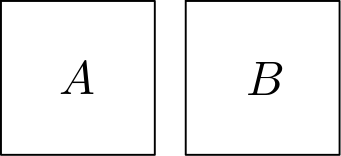
\includegraphics[width=.45\textwidth,height=.07\textheight]{MNG_AB}
\end{minipage}
\begin{minipage}[height=.1\textheight]{.45\textwidth}
\centering
\small{\texttt{(b)}} \\
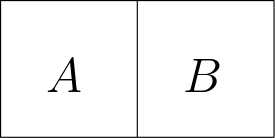
\includegraphics[width=.45\textwidth,height=.07\textheight]{MNG_ABx}
\end{minipage}
\caption{ \label{fig:MNGspaceglue}
Depiction of spatial gluing for \twots\ with spatial translation symmetry.
(a) Initial \twots\ and (b) \twots\ with correct gluing order.
}
\end{figure}


\begin{figure}
\begin{minipage}[height=.1\textheight]{.45\textwidth}
\centering
\small{\texttt{(a)}} \\
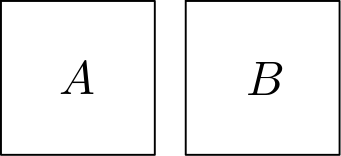
\includegraphics[width=.45\textwidth,height=.07\textheight]{MNG_AB}
\end{minipage}
\begin{minipage}[height=.1\textheight]{.45\textwidth}
\centering
\small{\texttt{(b)}} \\
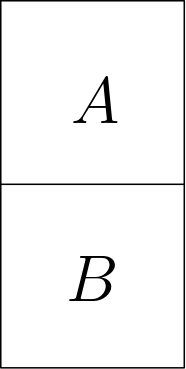
\includegraphics[width=.225\textwidth,height=.15\textheight]{MNG_ABt}
\end{minipage}
\caption{ \label{fig:MNGtimeglue}
Depiction of temporal gluing for \twots\ with either spatial translation symmetry
or reflection symmetry. (a) Initial
\twots\ and (b) \twots\ with correct gluing order.
}
\end{figure}


\begin{figure}
\begin{minipage}[height=.1\textheight]{.45\textwidth}
\centering
\small{\texttt{(a)}} \\
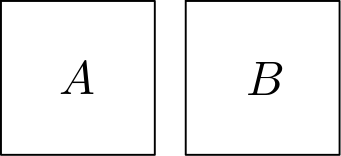
\includegraphics[width=.45\textwidth,height=.07\textheight]{MNG_AB}
\end{minipage}
\begin{minipage}[height=.1\textheight]{.45\textwidth}
\centering
\small{\texttt{(b)}} \\
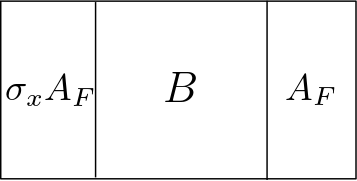
\includegraphics[width=.45\textwidth,height=.07\textheight]{MNG_ABreflx}
\end{minipage}
\caption{ \label{fig:MNGreflxglue}
Depiction of spatial gluing for \twots\ with reflection symmetry. (a) Initial
\twots\ and (b) \twots\ with correct gluing order.
}
\end{figure}


\begin{figure}
\begin{minipage}[height=.1\textheight]{.45\textwidth}
\centering
\small{\texttt{(a)}} \\
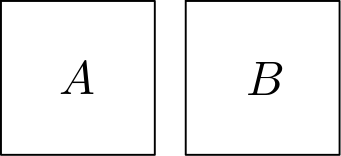
\includegraphics[width=.45\textwidth,height=.07\textheight]{MNG_AB}
\end{minipage}
\begin{minipage}[height=.1\textheight]{.45\textwidth}
\centering
\small{\texttt{(b)}} \\
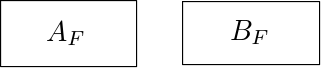
\includegraphics[width=.5\textwidth,height=.035\textheight]{MNG_AFBFshiftrefl}
\end{minipage}
\centering
\begin{minipage}[height=.1\textheight]{.6\textwidth}
\centering
\small{\texttt{(c)}} \\
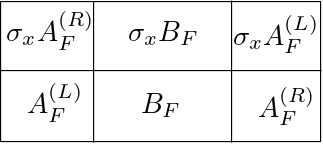
\includegraphics[width=.45\textwidth,height=.09\textheight]{MNG_ABshiftreflx}
\end{minipage}
\caption{ \label{fig:MNGshiftreflxglue}
Depiction of spatial gluing for \twots\ with shift-reflection symmetry. (a) Initial
\twots\ and (b)fundamental symmetry domains (c) post-gluing initial condition for
shift-reflection \twot. Superscripts in this instance stand for ``left'' and
``right'' halves of the corresponding fundamental domain $A_F$
}
\end{figure}

\begin{figure}
\begin{minipage}[height=.1\textheight]{.45\textwidth}
\centering
\small{\texttt{(a)}} \\
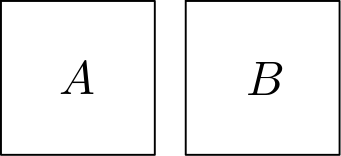
\includegraphics[width=.45\textwidth,height=.07\textheight]{MNG_AB}
\end{minipage}
\begin{minipage}[height=.1\textheight]{.45\textwidth}
\centering
\small{\texttt{(b)}} \\
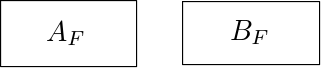
\includegraphics[width=.5\textwidth,height=.035\textheight]{MNG_AFBFshiftrefl}
\end{minipage}
\centering
\begin{minipage}[height=.1\textheight]{.45\textwidth}
\centering
\small{\texttt{(c)}} \\
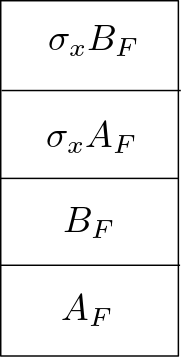
\includegraphics[width=.25\textwidth,height=.20\textheight]{MNG_ABshiftreflt}
\end{minipage}
\caption{ \label{fig:MNGshiftrefltglue}
Depiction of temporal gluing for \twots\ with shift-reflection symmetry. (a) Initial
\twots\ (b) fundamental symmetry domains and (c) post-gluing initial condition for
shift-reflection \twot.
}
\end{figure}

\begin{figure}
\centering
\begin{minipage}[height=.4\textheight]{.66\textwidth}
\centering
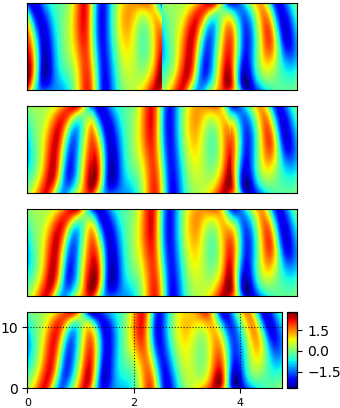
\includegraphics[width=.7\textwidth,height=.6\textheight]{MNGppo12space_glue}
\end{minipage}
\caption{ \label{fig:MNGppo12spaceglue}
Spatial gluing of the two shortest shift-reflection
\twots. The sizes of the fundamental domains of these
\twots\ are
$[\speriod{1},\period{1}]=[3.5\cdots,20.50\cdots]$
and
$[\speriod{2},\period{2}]=[3.5\cdots,28.66\cdots]$
respectively.
The result is a
shift-reflection \twot\ with
$[\speriod{1,2},\period{1,2}]=[6.79\cdots,24.82\cdots]$
fundamental domain.
}
\end{figure}


\begin{figure}
\begin{minipage}[height=.4\textheight]{.99\textwidth}
\centering
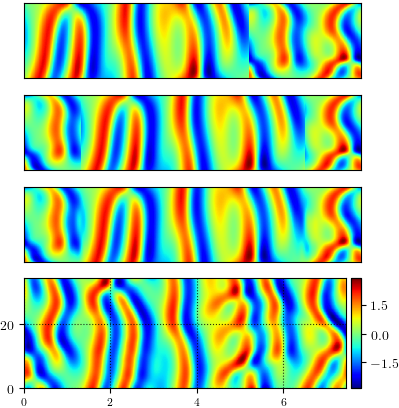
\includegraphics[width=.99\textwidth,height=.66\textheight]{MNGppo123space_glue}
\end{minipage}
\caption{ \label{fig:ppo123spaceglue}
Gluing procedure which spatially combines the third shortest (period) shift-reflection
invariant
$[\speriod{3},\period{3}]=[3.5\cdots,64.70\cdots]$
\twot\
 with the resultant shift-reflection invariant \twot\
from
\PCedit{reffig{fig:ppo12spaceglue}} %2019-12-06
with
$[\speriod{1,2},\period{1,2}]=[6.79\cdots,24.82\cdots]$
fundamental domain.
This results in another shift-reflection
\twot\ with the
$[\speriod{1,2,3},\period{1,2,3}]=[10.53\cdots,68.84\cdots]$
 fundamental domain.
The dramatic change between the last
two panels is presumably an effect of the
discrepancy between the temporal period of
the constituent solutions.
}
\end{figure}


\begin{figure}
\centering
\begin{minipage}[height=.4\textheight]{.66\textwidth}
\centering
\includegraphics[width=.7\textwidth,height=.6\textheight]{MNG_ppolargeTspaceglue}
\end{minipage}
\caption{ \label{fig:MNGppo12spaceglue1}
Spatial gluing of the two shortest shift-reflection
\twots. The sizes of the fundamental domains of these
\twots\ are
$[\speriod{1},\period{1}]=[3.5\cdots,20.50\cdots]$
and
$[\speriod{2},\period{2}]=[3.5\cdots,28.66\cdots]$
respectively.
The result is a
shift-reflection \twot\ with
$[\speriod{1,2},\period{1,2}]=[6.79\cdots,24.82\cdots]$
fundamental domain.
}
\end{figure}


\begin{figure}
\centering
\begin{minipage}[height=.4\textheight]{.66\textwidth}
\centering
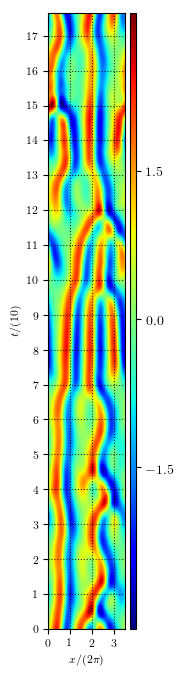
\includegraphics[width=.7\textwidth,height=.6\textheight]{MNG_rpoLargeTtimeglue}
\end{minipage}
\caption{ \label{fig:MNGppo12spaceglue2}
Spatial gluing of the two shortest shift-reflection
\twots. The sizes of the fundamental domains of these
\twots\ are
$[\speriod{1},\period{1}]=[3.5\cdots,20.50\cdots]$
and
$[\speriod{2},\period{2}]=[3.5\cdots,28.66\cdots]$
respectively.
The result is a
shift-reflection \twot\ with
$[\speriod{1,2},\period{1,2}]=[6.79\cdots,24.82\cdots]$
fundamental domain.
}
\end{figure}

and \reffig{fig:ppo123spaceglue}
both demonstrate the spatial gluing
of shift-reflection \twots. In fact, \reffig{fig:ppo123spaceglue}
uses the result of

as an initial
condition. We chose to display these two gluing examples
because they are demonstrative of how gluing can be performed
iteratively to find progressively larger solutions.

Our tiling and gluing methods constitute ways that larger \twots\
can be found by utilizing smaller \twots. This notion of combinations
has been performed temporally\rf{DV03} as a natural
consequence of symbolic dynamics. In other words, for a dynamical system
with a chaotic attractor it is somewhat straightforward to interpret
symbolic itineraries; they represent visitation of different partitioned
areas of the attractor parameterized with time.
The idea to do this with
respect to spatial dimensions is desirable in the context of minimal
computational cells of plane Couette for instance. Combining solutions
in a \spt\ manner is a whole other beast as symbolic blocks are
hard to interpret in the context of state space.



As opposed to the more common Newton and GMRES methods. I think
The most promising of these numerical that I can try out are the
so called accelerated methods, which use the acceleration techniques
of the past derived by Nesterov\rf{Nesterov83}

applied to newer optimization algorithms.

Implemented a number of new numerical methods to see if any of them could
compete with what I currently have. Out of the three classes of solvers,
(descent methods, direct methods, iterative methods) iterative methods
have work terribly for me. Therefore in order to see if its just my innate
disability to be able to use these methods I am running a suite of tests
using built in optimization algorithms in SciPy.

On the other numerical front, I implemented two different types of Levenberg-Marquardt
algorithms, the first one\rf{FZlevmar13} performed much better than \refref{WHlevmar84},
and much better than the BiCGSTAB algorithm I also implemented; but for whatever
reason the Gauss-Newton with back-tracking performs better in all cases I have tried
so far.

I also tried more testing with the accelerated adjoint descent that I had recently forgone
in favor of using a lower order integration scheme in fictitious time with preconditioning,
I'm thinking I'll likely stick to that as well.

The main portion of today's work was to implement the gluing algorithm that takes any
two \twot\ solutions with the same solution and glues them together, with a slough of
options as to how one specifically wants to do this, namely, whether to concatenate in
space or time, whether to pad the boundaries between the two solutions with buffer
zones, and how to smooth out the glued together data. The smoothing still needs some fine
tuning; I'm using circular convolution with an anisotropic Gaussian that is wider in the
dimension by which two solutions were glued. Currently trying to run through some test
cases. The two shortest \ppo\ solutions concatenated in time after adjoint descent
looks interesting but Gauss-Newton squashes it into an equilibrium. Definitely needs
some more fine tuning on the smoothing front.

Worked on symbolic dynamic initial condition
generation and thinking through gluing codes

The general idea is to take the library of solutions that I have found
and then automate the process that glues them together; \ie
the automation will contain the following subroutines:
\begin{enumerate}
\item Determine symmetry subgroup of the solutions.
\item Choose solutions and direction (space or time) to glue.
\item Make sure the discretizations match such that the final result
is a rectangular grid.
\item Use Fourier smoothing, Gaussian mollifiers, or insertion of
zeros to pad the two solutions and connect them or any combination
of these procedures.
\item Determine $(\speriod{},\period{},\sigma)$ based on averaging.
\item Use either hybrid adjoint-descent Newton or adjoint descent
Newton Krylov to converge the approximate solution.
\end{enumerate}

I have an inkling that liberal use of inserting streaks and traveling
wave type solutions might be used to help glue solutions together as
but I don't have motivation for this other than intuition currently.

\begin{figure}
\begin{minipage}[height=.30\textheight]{.6\textwidth}
\centering \small{\texttt{(a)}}\\
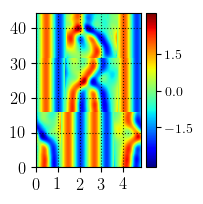
\includegraphics[width=.8\textwidth,height=.3\textheight]{MNG_ppo_tiling_init_pretruncation_1}
\end{minipage}
\begin{minipage}[height=.30\textheight]{.6\textwidth}
\centering \small{\texttt{(b)}}\\
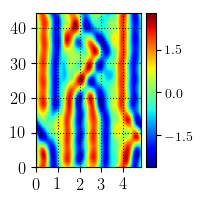
\includegraphics[width=.8\textwidth,height=.3\textheight]{MNG_ppo_tiling_init_1}
\end{minipage}
\begin{minipage}[height=.30\textheight]{.6\textwidth}
\centering \small{\texttt{(c)}}\\
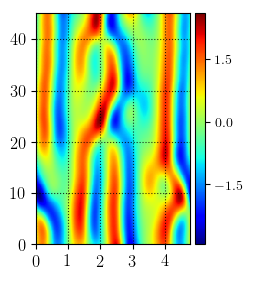
\includegraphics[width=.7\textwidth,height=.3\textheight]{MNG_ppo_tiling_final_1}
\end{minipage}
\begin{minipage}[height=.30\textheight]{.6\textwidth}
\centering \small{\texttt{(d)}}\\
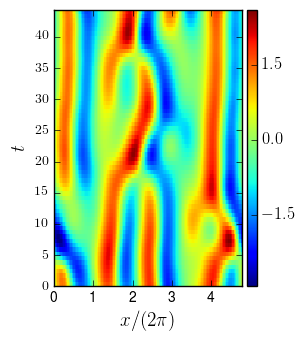
\includegraphics[width=.75\textwidth,height=.3\textheight]{MNG_ppo_L30_T44}
\end{minipage}
\caption{ \label{fig:MNG_ppotiling_one}
(a) Gluing together the three subdomains from \reffig{fig:MNG_pposubdomains_zero}
in the temporal direction. This is the initial condition for the fundamental domain
of a \twot\ with shift-reflection symmetry.
(b) The convergent result of the numerics with initial condition (a).
(c) \reffig{fig:MNG_frankenstein}
 %\emph{ppo\_L30\_T44}
included for comparison to (b).
}
\end{figure}



After last week's plumbers union meeting I had a conversation with Michael Krygier, who works mostly
on numerical Taylor-Couette. We had a chat that inspired me to get back into investigating iterative methods
and I had an epiphany. My the truth was obscured because of the conventional computation in the literature, almost
everyone in the field that uses Newton-Krylov or other iterative methods
approximates $J^t \delta x \approx \frac{F^{t+\delta t}(x+\delta x)-F^t(x)}{|\delta x|}$. It's due to the fact that I
had seen this equation or approximation ubiquitously that I was blinded to a \emph{far} better way of performing
this computation, one that in fact \emph{I already use in the adjoint descent!}.
Namely, because the dependence on
$T$ is completely explicit in the spatiotemporal \KSe\ and doesn't rely on
implicit forward-time mappings (\ie time-integration),
all I have to do is compute the action of the matrix
$J = \frac{\partial F}{\partial x}$ on a vector $\delta x$! I can't believe
I haven't realized this until today. It's literally (up to a transpose)
how I've been employing the adjoint descent method
for many months now, but like I said the literature blinded
me I suppose.

What I mean by ``compute the action of the matrix $J$ on a vector $\delta x$''
is to decompose the matrix multiplications
into elementwise operations dependent on the spatiotemporal
Fourier mode indices. It's actually ridiculously easy and I'm just baffled
but how I didn't see it when it was right in front of my eyes.
The mathematical equation that follows is,

\beq
J\cdot x = (\ii \omegaj -q_m^2 + q_m^4 + \frac{\ii q_m S}{T})x_{n,m} + \ii q_m \mathcal{F}diag(u)\mathcal{F}^{-1}x \,.
\eeq

Such an equation can be evaluated without the use of any matrices whatsoever (the linear term with $S$ is for solutions with continuous
symmetry. There is no error or approximation (up to machine precision)
by performing the calculation in this matrix-free way (yet another boon of spatiotemporal formulation), such that the application
translates nicely to iterative methods that require the matrix-vector product, such as Newton-Krylov-Hookstep.

%mess ups of gluing strips and buffers



The reason for this is that although the smoothing
of the piecewise linear functions would result in
a continuous field that would like the constituent
\twots\ together the tangent space would be terribly
wrong. I attribute the success of the gluing in spite
of this to the potency of the \spt\ numerical methods (adjoint
descent, etc.)

I will propose an improvement (whose implementation
I will reserve for after the paper is written due to
the amount of work involved).

The method by which I believe that solutions should be
glued, or at least the initial \twots\ should be
joined is to solve a supplementary problem which
fills in a zero padded region by virtue of approximately
solving the BVP problem induced by the connection of the boundaries
of each \twot.

Specifically, because we are more concerned with the
tangent space being correct we will utilize Neumann
boundary conditions for the BVP. Because of these
boundary conditions the ``natural'' choice for the
discretization of this connecting region is to
either used finite difference methods or
Chebyshev collocation methods. The former
is rather expedient and perhaps would be better
for this additional optimization problem because
it will not result in an exact solution either way.

The reason we know that the intermediate area
cannot have a tangent space that satisfies the \KSe\
everywhere locally is because we are connecting two
\twot\ solutions. For instance, integration of the
IVP initiated at either boundary would (theoretically)
result in the \twot\ being repeated ad infinitum.

There is still indecision on my part as to the
precise method by which the problem could be solved.

The first, a fully \spt\ method, would allow for
use of the currently implemented (with modifications
to incorporate the boundary conditions) numerical
methods. The idea is to merely follow the typical
procedure except the basis would be either Fourier-Chebyshev
or Chebyshev-Fourier depending on the gluing direction.

The second (more straightforward in my mind) method
would be to apply the variational Newton descent formalism
to a Chebyshev basis with Neumann BC. This would be
easily accomplished by using a Chebyshev basis and
differentiation operator instead of the finite difference
methods. The only difference between the spatial gluing
and temporal gluing cases would then be
the tangent space equations,
namely, whether we are using \refeq{e-Fks} or \refeq{e-ksX}
in the variational Newton descent equation.

As I'm writing this I don't think the \spt\ method would
really be that difficult. The only difference from the
current \spt\ method would be to incorporate Chebyshev
transforms and modify the differential
operators to accomodate the boundary conditions.
For instance, if tackling Neumann BC
in time then for an $N$ by $M$ time by space discretization
(Fourier in space, Chebyshev in time) then the
correct form of the equation would take the spectral
coeff
Let $u_t(A)$ and $u_t(B)$ represent the first time
derivative evaluated on the ``boundary'' of each solution.
In matrix notation we have the following



Much like the clipping process used to find tiles combining solutions in space-time,
the overarching idea of gluing is straightforward and intuitive. We lean towards simplicity
such that the process of gluing and converging \twots\
is only slightly more complex than the original method of trawling for \twots.
With this in mind, what do we mean exactly when we say that we are gluing \twots?
As \twots\ are infinite space-time solutions the notion of gluing them doesn't
actually make sense; the actual entities being glued are the compact support
of these solutions. This is a familiar notion which has many different names:
Brillouin zone, fundamental domain, unit cell of a lattice, etc. To
distinguish between the infinite space-time \twots\ and their finite
representatives which we shall refer to as tiles.

The first step is to choose which \twots\ to glue and how to arrange them.
The general case is that we have a general $s_n \times s_m$ sized mosaic of tiles
with no particular attention given to whether or not the tiles fit well together.
The minimum requirement so that gluing is well defined operation is that
tiles must have equal number of grid points along boundaries being glued.
This creates a problem, however, as
different tiles will have different \spt\ dimensions $T,L$ because
they are fundamentally different solutions.
Therefore, the domains of each lattice are
different but the number of grid points is the same, hence, the grid spacings
are necessarily different. This problem actually
helps provide a precise meaning to the term ``gluing''.
Gluing is a method of creating initial conditions via the combination
of \spt\ tiles which approximates the corresponding non-uniform rectangular lattice
as uniform. The regularization of the lattice is a global
transformation but it introduces error in
the form of local tangent space distortions which, of course,
depend on the local change in mesh size.
% Should I just remove the derivation and replace it with the result?
In Fourier space, differentiation
is equivalent to multiplication of the \Fcs\ by the corresponding
frequencies. Using this fact, we can create a crude bound on the error
introduced to give us an idea as to how detrimental the approximation
is. In a discrete setting, for a dimension of length $d$,
the greatest frequencies that are accounted for by an $N$ point discrete
Fourier transform are $\frac{2\pi N}{d}$. Therefore, the error between
an order $n$ tangent of the tile and its gluing approximation scales like
\beq
\partial_d^n u - \partial_d^n u' \sim (2\pi N)^n (\frac{1}{d^n} - \frac{1}{d'^{n}}) \utensor.
\eeq
By substituting $d' = d + \delta d$ and assuming $\delta d$ is small
\bea \nonumber
\Delta \partial_d^n \utensor &\sim& n \frac{\delta d}{d} \big( \frac{2\pi N}{d} \big)^n \utensor \continue
                    &\equiv& \frac{\partial [\partial_d^n u]}{\partial d} \delta d \,.
\eea
This result, while quite obvious in hindsight, would be different if we had been using finite
differences to compute the tangents.
Therefore the total error of the approximation can be found by the summation of the error
of each tile individually
\beq
\Delta F = \sum_z   (\delta L)_z \frac{\partial F}{\partial L}\Big|_{u = u_z}+
 (\delta T)_z\frac{\partial F}{\partial T}\Big|_{u = u_z}\,.
\eeq
We derived how the error depends on local changes to mesh size; we did not
however describe how to \emph{choose} the final mesh size.
The choice of the parameters depends on how the gluing is performed. We describe
two methods which differ in complexity there are a number of intermediate
states but these two examples get the point across.
The simplest method merely rediscretizes and concatenates the tiles, setting
the new dimensions to be the average of the tile dimensions. Note that this averaging
should only occur with respect to the dimension transverse to the gluing.
For example, if gluing two tiles together in time, the period would be
$T = T_1 + T_2$ but the spatial period would be $L = \frac{L_1 + L_2}{2}$.
In this case, the number of spatial grid points and the temporal grid spacing
need to be the same. This same idea can be extended to arbitrary sized gluings;
generalizing to a summation over the tiles
\bea
T &=& \frac{1}{s_x}\sum_{i,j=1,1}^{s_x, s_t} T_{ij} \continue
L &=& \frac{1}{s_t}\sum_{i,j=1,1}^{s_x, s_t} L_{ij} \,.
\eea
The more complicated alternative is to glue tiles in a pairwise fashion, building
block by block. The problem with this method is that it is not agnostic to the order
in which tiles are being glued as each iteration requires lattice regularization.
For example, gluing four tiles together spatially would be completed in three pairwise steps;
this results in the final approximation having period
\beq
T = \sum_{i=1}^{s_x-1} \frac{T_i}{2^{s_x-i}}
\eeq
where the index $i$ represents the sequential gluing of tiles. Going even further,
we can alternate between gluing and converging; this allows for much more complicated
strategies for gluing such as gluing tiles together in ascending order of \spt\ domain size.
The motivation for doing so is that even though there are no dynamical instabilities, the difficulty
of finding \twots\ still scales with their \spt\ domain size. Note that this process does not
need to be done from scratch for each gluing; once converged, the result can be saved for later usage.
As can be seen the options seem to only limited by our creativity, we opt for simple solutions
as we have not developed any best practices as of yet. Before any more improvements can be discussed
we first need to deciminate the results of the methods proposed thus far.


\begin{figure}
\begin{minipage}[height=.4\textheight]{.5\textwidth}
\centering \small{\texttt{(a)}}\\
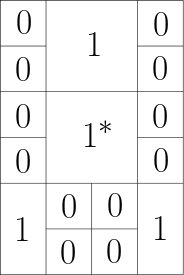
\includegraphics[width=.5\textwidth,height=.25\textheight]{MNG_symbolicblock}
\end{minipage}
\begin{minipage}[height=.4\textheight]{.5\textwidth}
\centering \small{\texttt{(b)}}\\
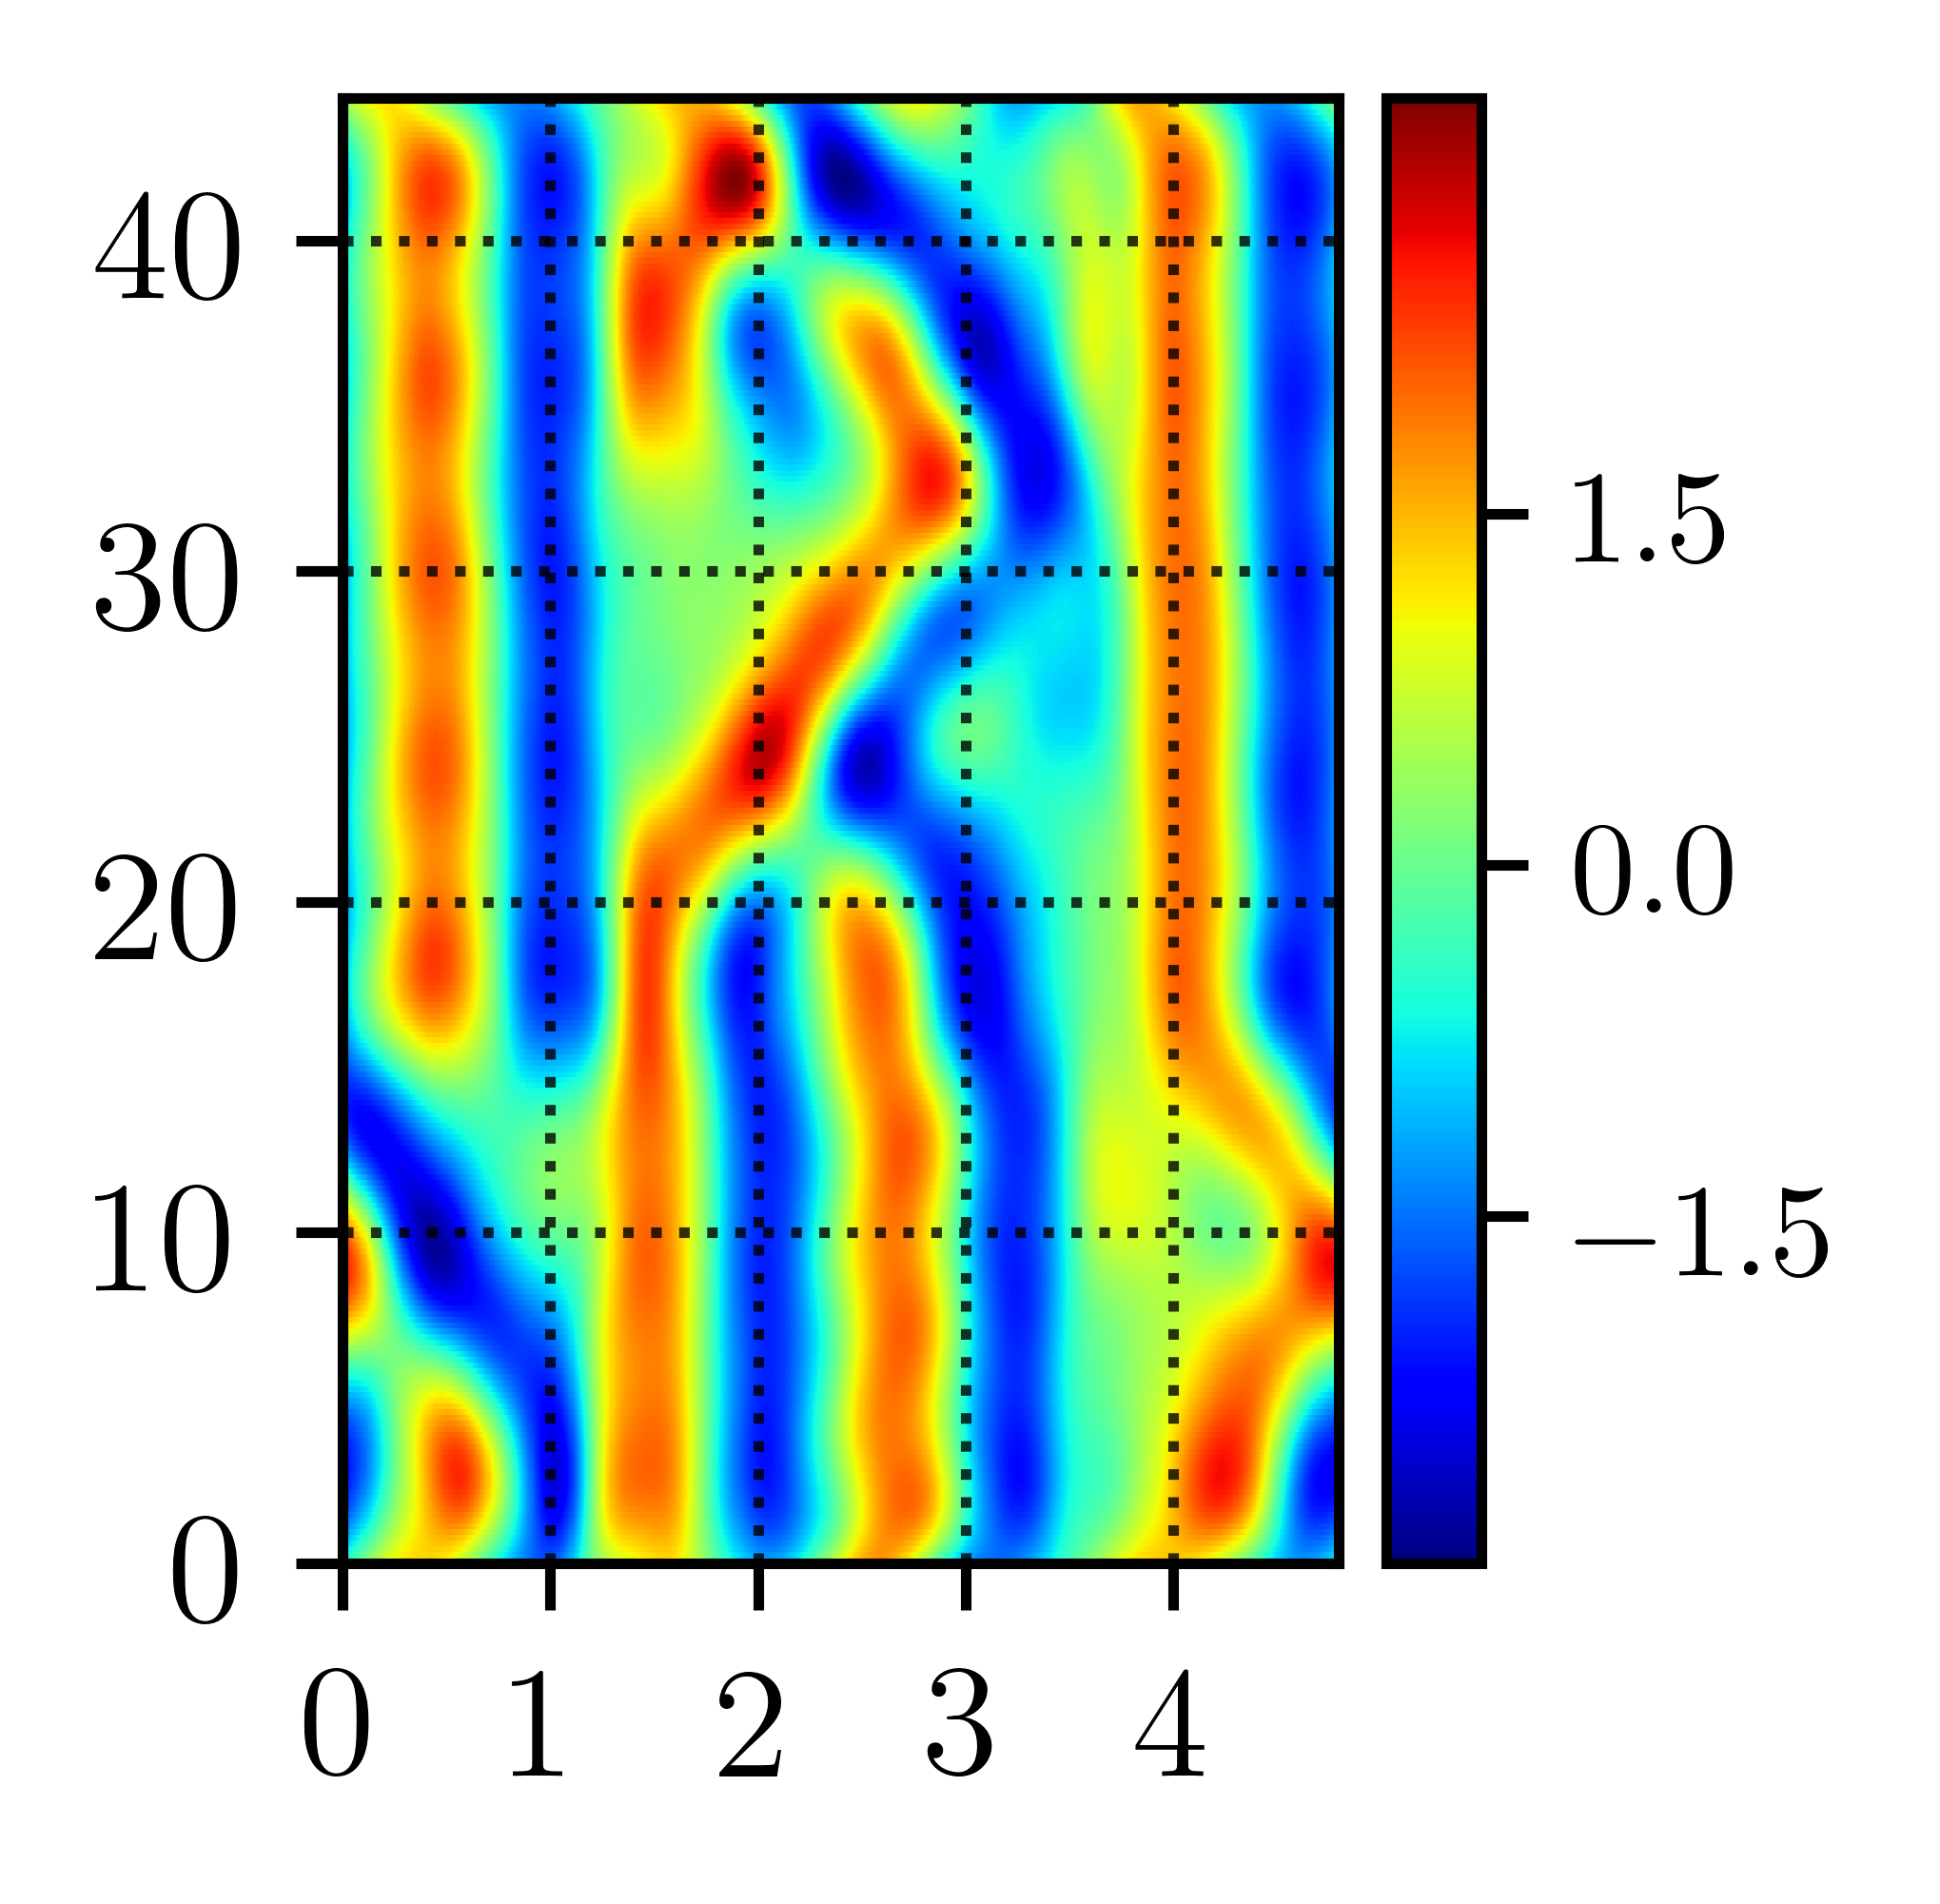
\includegraphics[width=.7\textwidth,height=.32\textheight]{MNG_trinary_initial}
\end{minipage}
\begin{minipage}[height=.4\textheight]{.5\textwidth}
\centering \small{\texttt{(c)}}\\
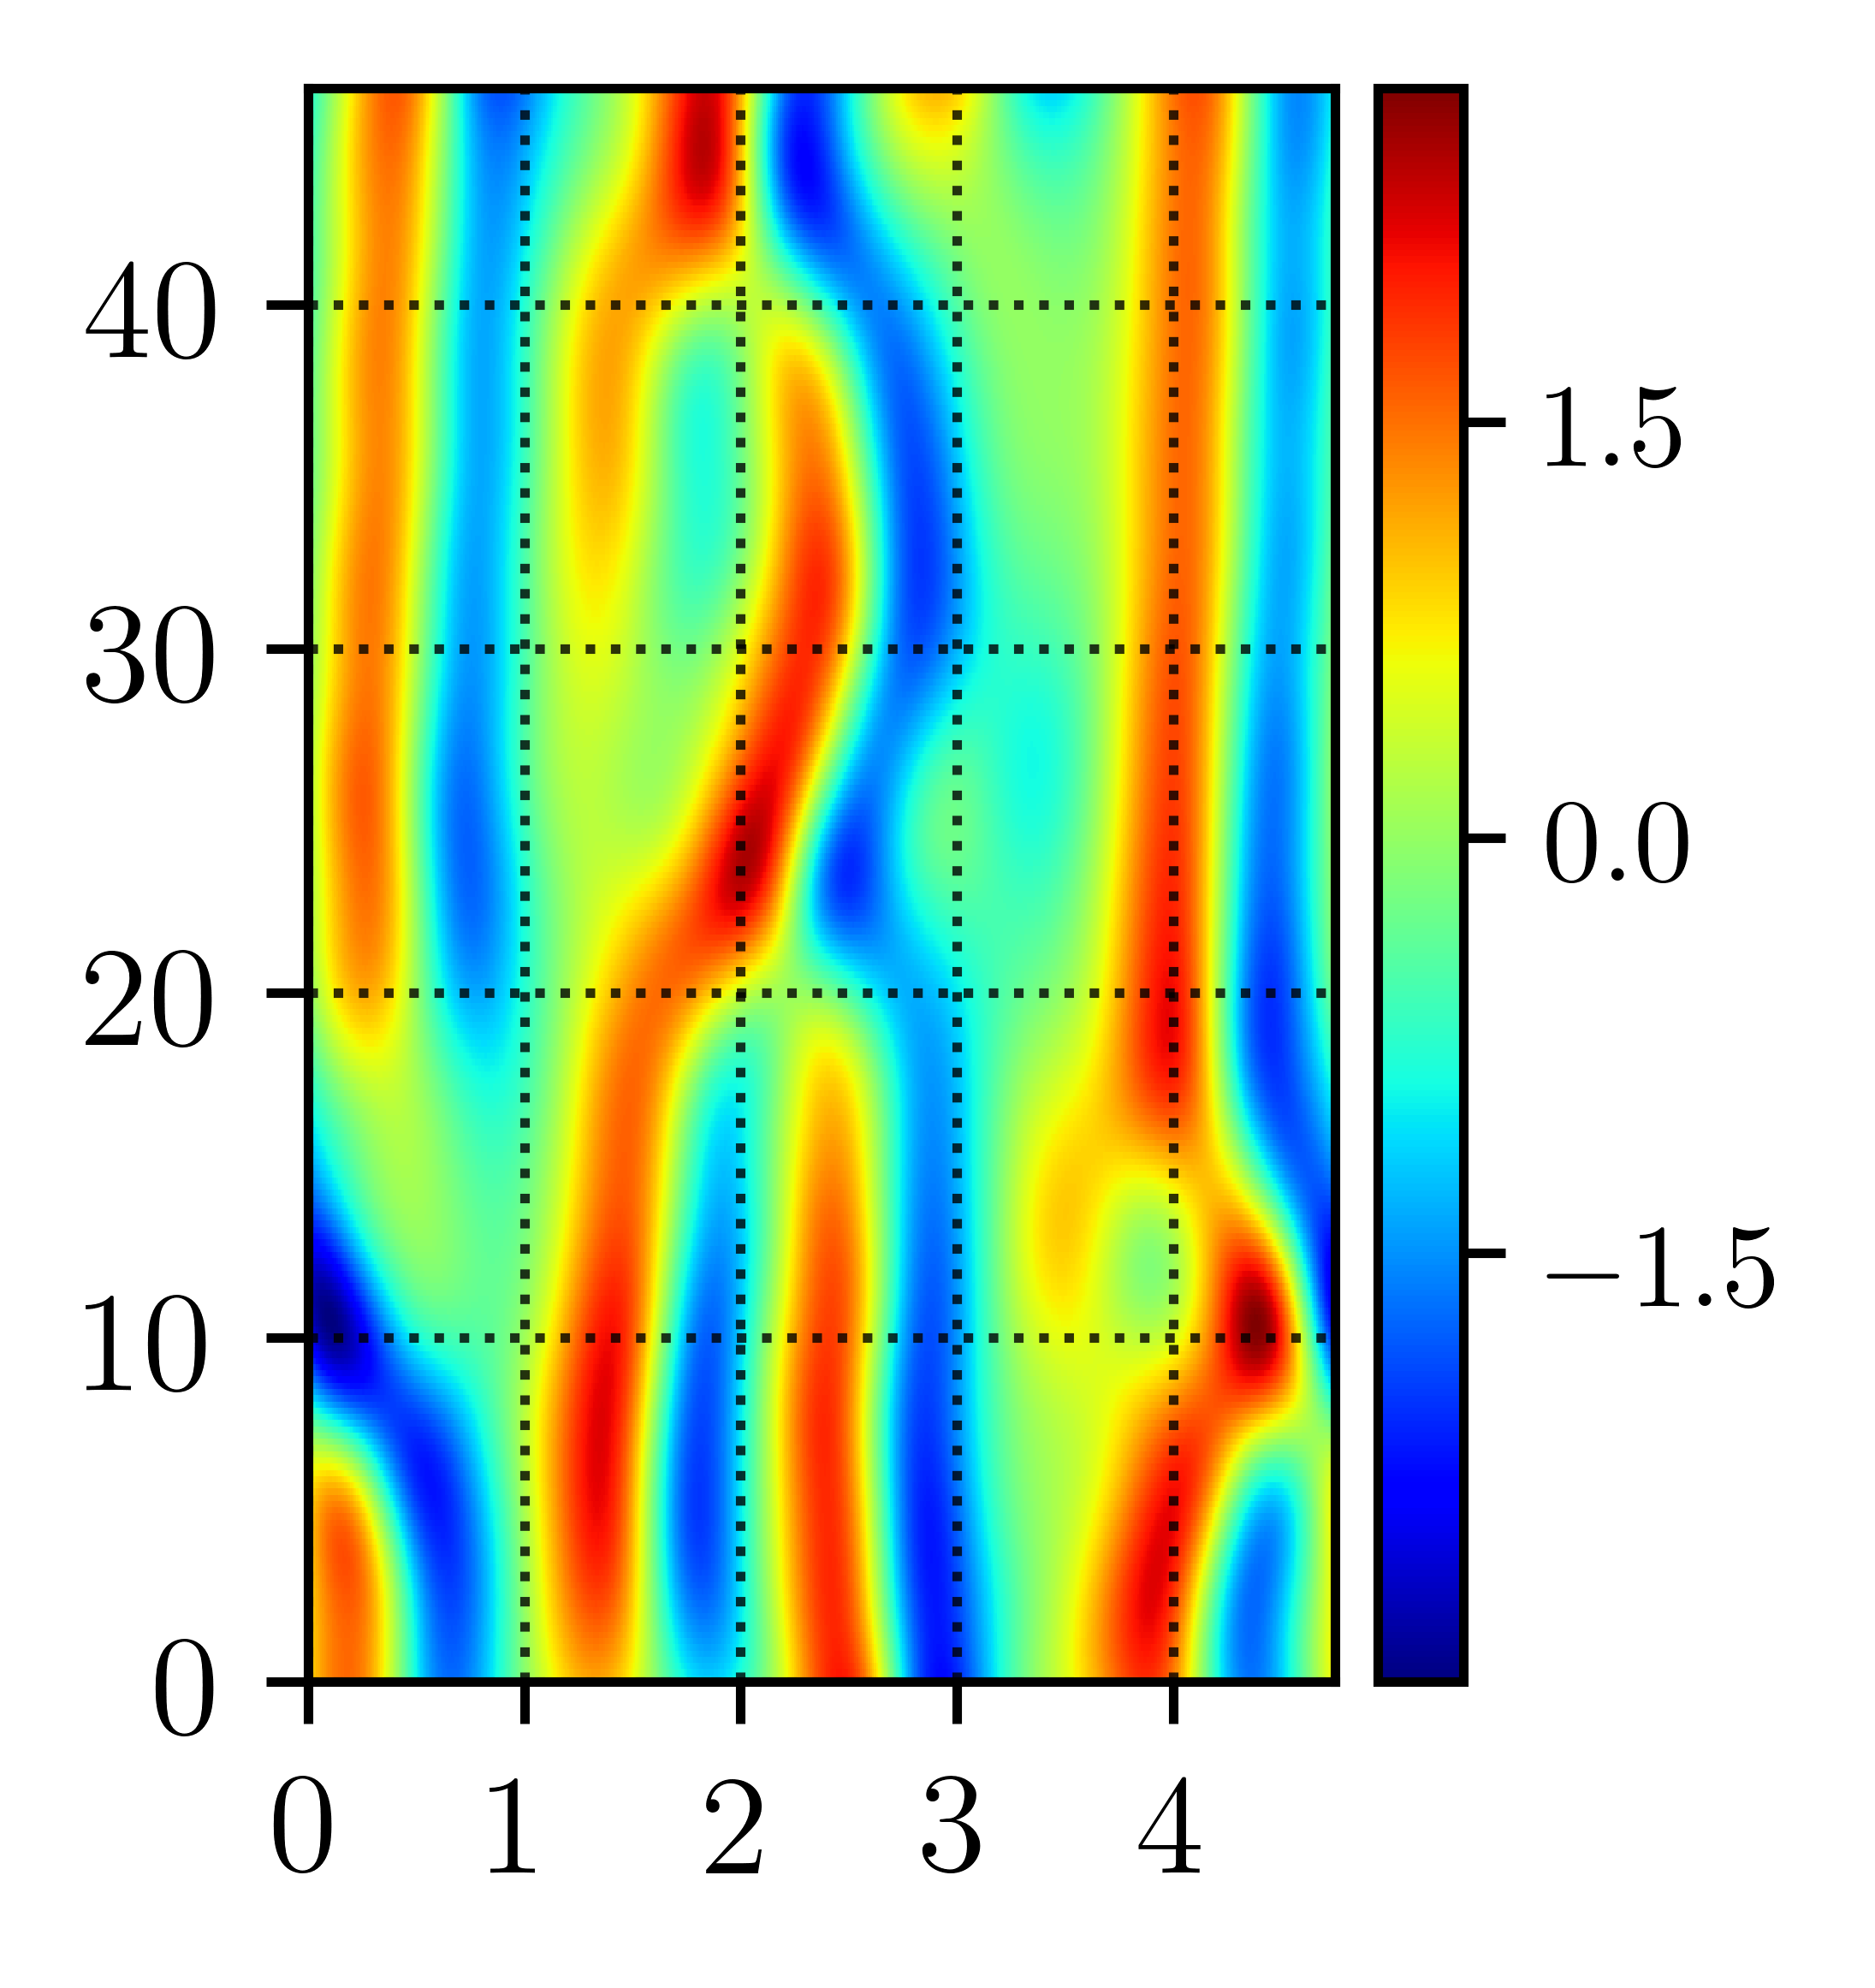
\includegraphics[width=.7\textwidth,height=.32\textheight]{MNG_trinary_final}
\end{minipage}
\begin{minipage}[height=.4\textheight]{.5\textwidth}
\centering \small{\texttt{(d)}}\\
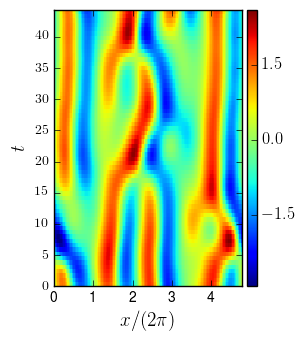
\includegraphics[width=.7\textwidth,height=.32\textheight]{MNG_ppo_L30_T44}
\end{minipage}
\caption{ \label{fig:trinarytiling}
(a) \Spt\ symbolic block representation created using group orbits
of three tile families,
(b) initial condition produced by combining tiles according to (a);
dimensions initialized at $[\speriod{b},\period{b}]=[4.79\cdots,88.62\cdots]$,
(c) converged \twot\ when using (b) as an initial condition,
(d) targeted \twot\ which (c) was trying to match.
}
\end{figure}

\MNGedit{Gluing proceeds as follows: select an array of {\fpo}s to glue
together (imagine creating a puzzle, wherein the pieces are {\fpo}s). Next, numerically
join this array of {\fpo}s together at their boundaries. This creates an initial guess whose
state is a patchwork of {\fpo} states and whose periods
are combinations of {\fpo} periods. As a last step, the discontinuities
of in the field are smoothed via truncation of the high frequency {\spt} {\Fcs}.}


%\subsubsection{glue}
It is one thing to claim that certain \spt\ \twots\ are the building blocks
of turbulence for the \KSe. It is
another thing entirely to put our money where our mouth is by actually using them in this manner. We would like to remind the audience that the ability to construct and find solutions in this manner
has not been witnessed in the literature. With this in mind our choices should
be treated as preliminary ones; it is entirely possible and likely that
many improvements could be made.
Much like the clipping process used to find tiles combining solutions in space-time,
the overarching idea of gluing is straightforward and intuitive.
Specifically, the tiles represent the
Brillouin zone, fundamental domain, unit cell of a lattice, etc.
of each fundamental \twot.
The general case is that we have a general $s_n \times s_m$ sized mosaic of tiles.
The admissibility of the gluing is determined by the (currently unknown) symbolic
dynamics. Gluing is only well defined if the lattices being combined have the same
number of grid points along the gluing boundary.
This creates a problem, however, as
different tiles will have different \spt\ dimensions $\speriod{},\period{}$ because
they are fundamentally different solutions.
This actually helps provide a precise meaning to the term ``gluing''.
Gluing is a method of creating initial conditions which approximates
a non-uniform rectangular lattice (combination of tiles) as uniform.
This of course introduces local error which depends on the grid size; therefore
there should not be an extreme discrepancy between the \twots\ or tiles being glued.
With this in mind, we simply rediscretize and concatenate the new lattices.
The dimensions of the new lattice are determined by the sum or average of
the original dimensions.
For example, if gluing two tiles together in time, the new period would be
$\period{} = \period{1} + \period{2}$ but the new spatial period is
$\speriod{} = \frac{\speriod{1} + \speriod{2}}{2}$.
In this case the number of spatial grid \emph{points} and temporal grid \emph{spacing}
should be the same. There are many more complicated alternatives, limited only by
the imagination.

